\section{Analysis}
We conduct several analyses to anchor our observations. 
In \autoref{sec:analysis_noise}, We examine how architectural choices affect the balance between phonotactics and acoustics, echoing with evaluation results.
In \autoref{sec:analysis_phoneinv}, we study multilingual generalization and confirm that encoder-only architectures trained with diverse language coverage at all stages perform well for PR. 
In \autoref{sec:analysis_geo}, we analyze TP in detail and show that it effectively captures phone distribution differences across regions. 
Finally, in \autoref{sec:mallm}, we assess zero-shot performance of LALMs on challenging tasks, concluding that they remain insensitive to sociophonetic variation.

\subsection{Phonotactics or the Acoustic Signal}
\label{sec:analysis_noise}

\begin{figure}
    \centering
    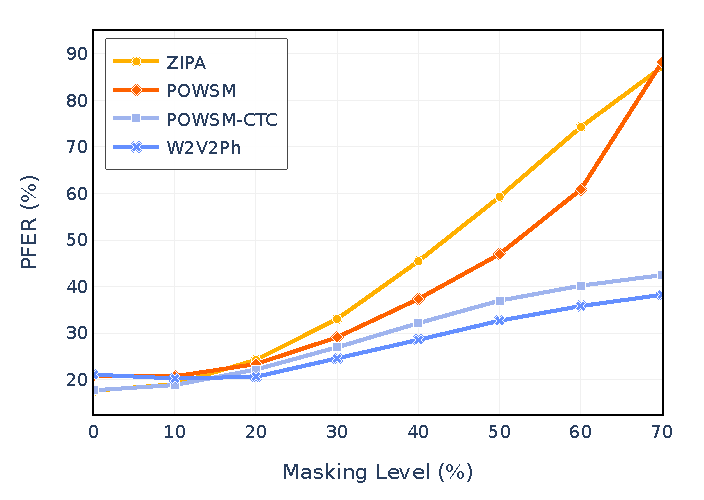
\includegraphics[width=\columnwidth]{figures/rq1_viz.pdf}
    \caption{PFER vs Phone masking rate. A PR model that relies only on acoustics should produce a horizontal line. Encoder-only models trained with CTC loss retain acoustic fidelity at high masking levels. See \autoref{sec:analysis_noise}.
    }
    \label{fig:fervsnoise}
    \vspace{-1em}
\end{figure}

Ideally, PR systems would faithfully transcribe the actual pronunciation in the speech signal via acoustic modeling.
Instead, model transcriptions often normalize toward standard pronunciations or other probabilistically likely phone patterns \citep{zipa,powsm}, essentially relying on (phone-level) language modeling \citep{pimentel2020phonotactic}.\footnote{A common example of such phonotactic knowledge is the intuition that \textit{brick} [\textipa{b\*rIk}] is a valid phone sequence in English while \textit{bnick} [\textipa{bnIk}] is not \citep{spe}.}
Additionally, models can also overfit phonotactics from the high-resource languages.
In this experiment, we investigate the extent to which PR systems rely on such phonotactic patterns present in the training data, as opposed to information derived directly from acoustic signal.

Using TIMIT \cite{garofolo1993timit}'s time-aligned phone transcripts, we replace $p\%$ of phones with silence, transcribe the modified speech using PR, and compute PFER against a reference containing only the remaining phones.
In \autoref{fig:fervsnoise}, we plot the phone masking rate against the PFER for different model families.
For a model that only relies on the acoustic waveform for prediction, the curve would be a horizontal line.
However, for models that rely on phonotactics, the PFER will increase with greater noise.
While all models start at a similar PFER, Wav2Vec2Phs and \powsmctc perform better than ZIPAs and \powsm at higher masking levels. Thus  \textbf{Wav2Vec2Phs relies more on the acoustic signal} than on phonotactics.
While \powsm is an AED model trained with next-token prediction, Wav2Vec2Phs and \powsmctc are encoder-only models trained with the CTC objective.

However, ZIPAs are also encoder-only (Zipformer \cite{yao2023zipformer})  models, but they are trained with a consistency regularized CTC (CR-CTC) loss \cite{crctc}.
The high PFER of ZIPA  means that \textbf{CR-CTC loss biases the model to learn from both phonotactics and acoustics}.
We hypothesize that ZIPAs' Zipformer-based downsampling bottleneck can be another possible reason for ZIPA's high PFER.
We also observe that the insertion rates for different models follow the same trend as the curves in \autoref{fig:fervsnoise}, showing that POWSM and ZIPA produce phonetic transcriptions even when there is no input speech.
Interestingly, \zipactcns and \powsm perform best on unseen languages, but \powsm struggles with seen-language variation, and \zipactcns underperforms on pathological speech. This aligns with the idea that some tasks benefit from learned phonological patterns, while others depend more on capturing acoustic information.


\subsection{Zero-Shot Phonetic Inventory Induction}
\label{sec:analysis_phoneinv}
Identifying the inventory of phones in a new language is an important linguistic application and often an early step toward developing a standardized transcription system for it.
Such a task requires PR models to recognize phones correctly in unseen phonetic environments.
Therefore, it relies on the phonetic diversity the models have seen in the input speech signal during training.
We explore these behaviors in this set of experiments.

\begin{figure}
    \centering
    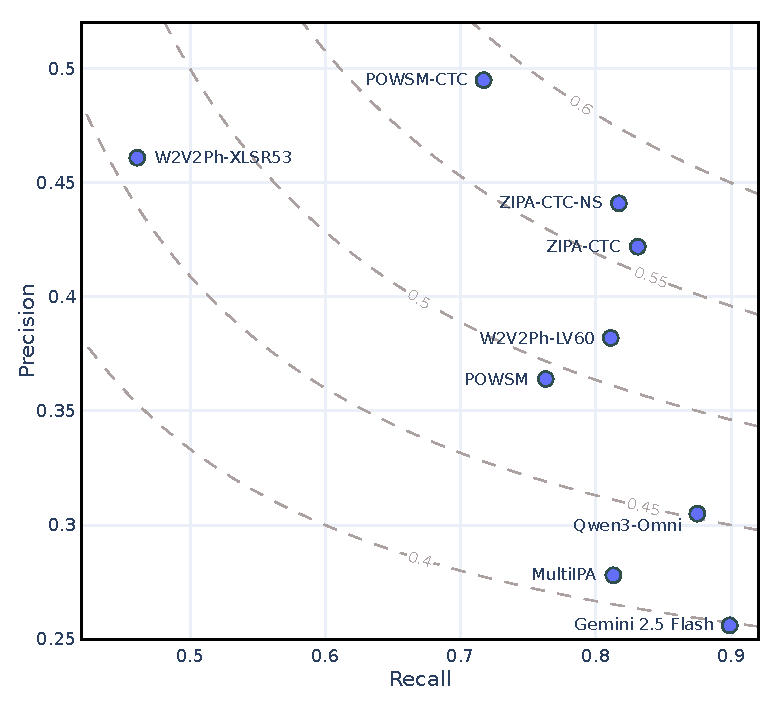
\includegraphics[width=\columnwidth]{figures/pr-scatter.pdf}
    \caption{Precision and Recall scores of PR systems on phone inventory induction for unseen languages (\autoref{sec:analysis_phoneinv}). CTC models trained with highly multilingual data are more stable.}
    \label{fig:inv_prec_recall}
    \vspace{-1em}
\end{figure}

Our dataset, derived from DoReCo, consists of low-resource languages absent from the training corpora of all models.
The transcripts from all models are used to compute the phone inventory after applying PanPhon-based phone tokenization \citep{panphon} followed by a set union over detected phones.
The ground truth inventory is constructed similarly using the phonetic transcriptions provided by DoReCo and set similarity metrics (\autoref{appendix:phoneinv}) are computed.
We show the macro-averaged values in \autoref{fig:inv_prec_recall}.

\powsmctc emerges as the strongest model.
The large gap between \powsmctc and \powsm (which differ only in architecture) suggests that the \textbf{encoder-only architecture plays a crucial role in high precision transcripts even in an unseen phonetic environment}.
As for ZIPAs, which differ in training data,  \zipactcns is more precise than \zipactc.
The extended multilingual training of \zipactcns on pseudo-labeled data leads to more precise phone predictions for unseen languages.
This suggests that noisy pseudo-labels allow for improved precision for new languages.
Similar trends is seen in comparing \xlsrf vs \lvsixty and \mipa, where multilingual SSL alone is insufficient for \mipa.
\textbf{Essentially, broader language coverage in both pre-training and supervised training result in a more precise model.}
Although the size of IPAPack++ (17k hr) is much smaller than that used for Wav2Vec2Phs (\textasciitilde160k hr), the larger number of languages in the supervised training stage (88 vs \textasciitilde40) leads to better recall for ZIPAs, compared to Wav2Vec2Phs.
This suggests that \textbf{diversity of languages is as important as the volume of data}.
Most models have a high recall ($>$ 70) and low precision ($<$ 50), suggesting that most predicted phones are incorrect and predictions have a high entropy.




\subsection{Geolocation for Dialectal Speech}
\label{sec:analysis_geo}
In \autoref{tab:phonebench:ext-results}, we observe that our TPs significantly outperform the RPs on Hindi dialectal geolocation \cite{foley-2024-geolocating}, where the former observes an average error of 146 km, while the latter observes an average error of 253 km.
As a reference, our data is spread over 1478 km (East-West) and 1703 km (North-South), covering the entire Hindi speaking region of India.
This performance is surprising, as the cascade-based approach loses suprasegmental information such as intonation that provide strong phonetic cues for the differentiation of dialects \citep{vicenik2013role, grabe2002intonational}. 
However, our results provide empirical evidence that morphological and phonetic differences suffice for fine-grained differentiation between Hindi dialects \citep{Gumperz1958PhonologicalDI}.
\begin{figure}
    \centering
    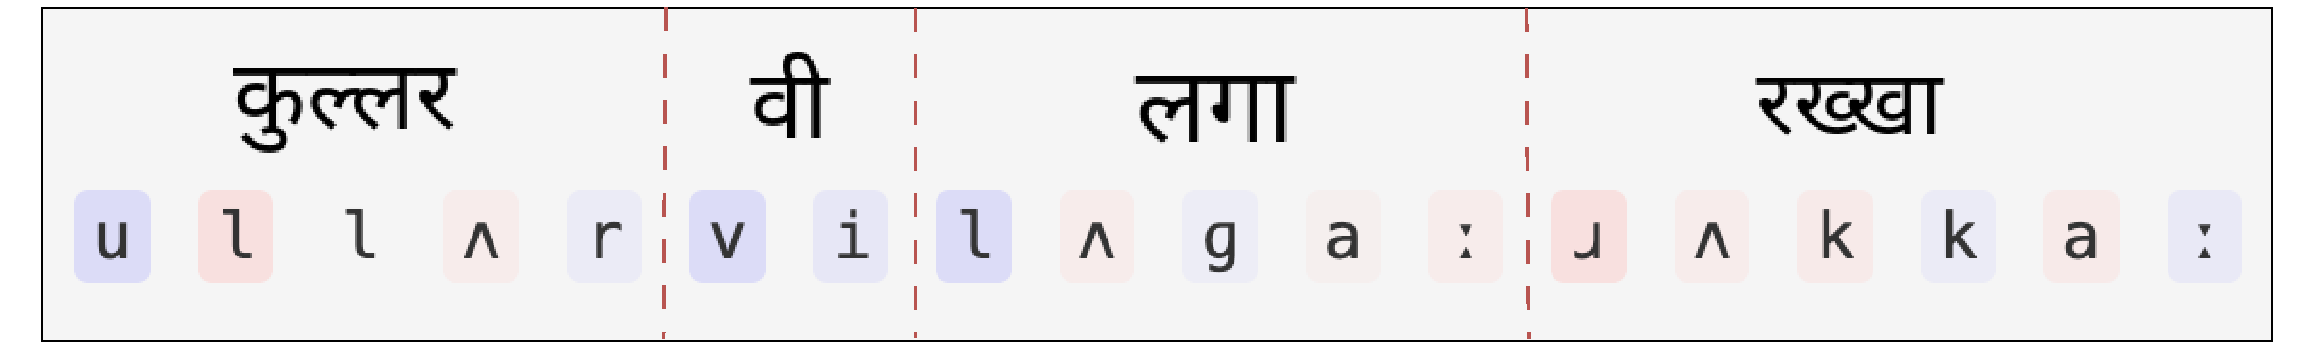
\includegraphics[width=\columnwidth]{figures/attribution2.pdf}
    \caption{Attribution map from Vaani \citep{vaani2025}. Red supports and blue opposes correct geolocation. \lvsixty detects doubled phones (\autoref{sec:analysis_geo}).}
    \vspace{-1em}
    \label{fig:attr}
\end{figure}

We hypothesize that part of the reason why hidden representations underperform cascade is also due to the downstream probe, where the RP employs attention pooling with an MLP, while the TP employs an RNN.
As the RNN preserves phone order information, even in the case where two dialects share similar phoneme inventories, \textbf{distributional differences of phone sequences between the dialects can be leveraged for fine-grained differentiation} \citep{Gumperz1958PhonologicalDI,shim2024phonotactic}.
We further analyze this behavior by employing integrated gradient based attribution maps \cite{sundararajan2017axiomatic} on TP.
There is a tendency of pronouncing two consonant sounds instead of one in the Bangru dialect of Haryanvi \cite{haryana}.
For example, the English loan word ``Cooler'' \textipa{[ku:lar]} becomes \textipa{[kullar]}, while the Hindi word ``Rakh\textipa{\=a}'' \textipa{[R@.k\super{h}a:]} (kept) becomes \textipa{[R@k.k\super{h}a:]}.
\autoref{fig:attr} shows attribution map for an utterance from \texttt{GEO-v}.
Speaker utters these words in their native accent, \lvsixty outputs \textipa{[ll]} and \textipa{[kk]}, and TP aligns with one of the doubled phones.
We leave a more detailed interpretability analysis to future work.


\subsection{LALMs lack phonetic perception}
\label{sec:mallm}
We examine the zero-shot predictions of LALMs on two tasks: \geov and \eda. 
On \geov, LALMs perform near chance level, whereas on \eda, \gemini achieves the strongest performance.

On \geov, both models exhibit geographic mode collapse. 
\qweni predicts New Delhi for nearly all inputs, while \gemini attains only 6.5\% hit@1 accuracy, with roughly 65\% of its predictions concentrated in 3–4 coordinate clusters near New Delhi (28.6°N, 77.2°E). 
This pattern suggests that \textbf{LALMs have limited sensitivity to dialectal variations} and are strongly biased toward higher-resourced dialects.

Similarly, on \eda, LALMs show a pronounced bias toward the Romance accent cluster, with 25.8\% of Slavic/Balkan and 28.5\% of South Asian accents misclassified as Romance.
Enabling thinking mode exacerbates rather than mitigates such biases by creating more attractor classes.
As a result, the F1-score on \eda drops from 32.7\% to 24.9\%.
Analysis of the reasoning traces reveals that the model over-relies on surface-level phonetic cues, mentioning ``Spanish/Italian/Portuguese'' in 87\% of erroneous Romance predictions and citing ``syllable-timed rhythm'' in 65\% of cases, leading to conflation of phonetically diverse accents.
The confusion matrices for both models are shown in \autoref{appendix:lalm-confusion}.
These findings suggest that LALMs lack the fine-grained acoustic perception, limiting their reliability for tasks requiring unbiased phonetic discrimination.